\section{解题思路}        
    \subsection{问题简介}
        \subsubsection{SAT问题}
            本问题称为``布尔表达式可满足性问题'',英文术语为``Boolean Satisfiability Problem'',该术语的Abbreviation是``SAT'' \par
                我们需要\textbf{解决的问题}是:对于一个布尔表达式(该布尔表达式由m个clause通过``$\cap$''组成,即$clause_{1} \cap \cdots \cap clause_{m}$),能否找到一组真值,使得该布尔表达式的赋值为真(即所有的$clause_{i}$都为true)\par
                拿一个简单的例子进行说明,现在我们考虑只有n=3个变量和m=1个clause的布尔表达式:

            \begin{center}
                $x_{1} \cup \overline{x_{2}} \cup x_{3}$
            \end{center}

            \par
            我们只需令:
        
            \begin{center}
                $x_{1}$ = true \quad $x_{2}$、$x_{3}$ 任意取
            \end{center}
            
            \par
            那么,该布尔表达式就为true
            \par
            一般地, 对于有n个变量和m个clause的布尔表达式:

            \begin{center}
                $clause_{1} = x_{1} \cup x_{2} \cup \cdots \cup x_{i} \cup \cdots \cup x_{n}$
            \end{center}
            
            \begin{center}
                $\vdots$
            \end{center}

            \begin{center}
                $clause_{l} = x_{1} \cup \overline{x_{2}} \cup \cdots \cup x_{i} \cup \cdots \cup x_{n}$
            \end{center}

            \begin{center}
                $\vdots$
            \end{center}

            \begin{center}
                $clause_{m} = x_{1} \cup \overline{x_{2}} \cup \cdots \cup \overline{x_{i}} \cup \cdots \cup x_{n}$
            \end{center}


            \par
            我们能不能找到一组真值,使得该布尔表达式的赋值为真呢?
            \par
            这就是我们接下来要讨论的``SAT''问题
        \subsubsection{K-SAT问题}
            那么什么是``K-SAT问题''呢?\par
                从定义上来讲,就是说我们使得布尔表达式中的每个clause只出现k个变量,我们拿一个其中一个$clause_{l}$进行说明:

        \begin{center}
            $clause_{l}=x_{1} \cup x_{2} \cup \cdots \cup x_{i} \cup \cdots \cup x_{j}$
        \end{center}

        \noindent{其中:}\par
            这个$clause_{l}$中出现的变量个数一共有k个,即$x_{1}\cdots x_{i} \cdots x_{j}$一共有k个\par
            这是什么意思呢?同样,我们拿一个简单的例子进行说明,考虑有n=5个变量和m=3个clause的布尔表达式:

        \begin{center}
            $x_{1} \cup \overline{x_{2}} \cup \overline{x_{3}} \cup x_{5}$
        \end{center}

        \begin{center}
            $x_{1} \cup x_{2} \cup x_{3} \cup x_{4}$
        \end{center}

        \begin{center}
            $x_{1} \cup x_{3} \cup x_{4} \cup x_{5}$
        \end{center}

        我们可以注意到一个事实:\\
        \begin{center}
            每个clause中出现的变量个数只有4个
        \end{center}
        \par
        很自然地,我们现在会有下面几个问题:\\
        \begin{center}
            我们不是已经定义了这个布尔表达式有n=5个变量吗?
        \end{center}
        \begin{center}
            为什么这个clause中出现的变量个数是4呢?
        \end{center}
        \begin{center}
            这个`4'代表了什么意思呢?
        \end{center}
            \par
        我们现在来进行回答:这个`4'实际上是``K-SAT问题''当中的K,换言之,在我们刚刚举的例子中,我们令K=4,也就是说,这是一个``K=4-SAT问题'',即``4-SAT问题''
        \subsubsection{3-SAT问题}
        同样,很自然地,我们回到要求解的问题当中,我们对给出的测例进行观察:

        \begin{center}
            $x_{1} \cup \overline{x_{2}} \cup \overline{x_{4}}$
        \end{center}

        \begin{center}
            $x_{2} \cup \overline{x_{3}} \cup x_{4}$
        \end{center}
        \begin{center}
            $x_{2} \cup x_{3} \cup x_{4}$
        \end{center}
        \begin{center}
            $x_{2} \cup x_{3} \cup \overline{x_{4}}$
        \end{center}
        \par
        我们可以注意到一个事实:\\
        \begin{center}
            每个clause中出现的变量个数只有3个
        \end{center}
        \par
        也就是说,我们需要解决的问题是一个``3-SAT问题''\\
        那么,如何进行求解呢?通过查询资料(已放在``参考文献''处),我们给出如下几种经典的解决方案:\par
            (1)回溯法 —— 最初尝试方式\par
            (2)DPLL算法 —— 主要实现方式\par
            (3)WalkSAT算法 —— 未尝试进行实现\\
        我们将在``解题方法简介''中进行解释
    \subsection{解题方法简介}
        ``SAT问题''的求解方法有很多,
        主要分为\underline{\textbf{完备性算法}}和非完备性算法,
        很自然地,我们会有两个问题:\\
        \begin{center}
            什么是``\underline{\textbf{完备性算法}}''?
        \end{center}
        \begin{center}
            什么是``非完备性算法''?
        \end{center}
        \par
        不太严谨地,我们拿一个例子进行说明:考虑有一张银行卡,它的密码有6位数字,但我们现在忘掉了它的密码,那么我们应该怎样试出这个银行卡的密码呢?\par
        很自然地,我们会有两种主要的尝试方案(不考虑其他外界因素):\\
        \begin{center}
            一个一个排列组合进行尝试
        \end{center}    
        \begin{center}
            灵光一现,想到一个密码,然后输入并且进行验证
        \end{center}
        \par
        我们认为:
        \begin{center}
            第(1)种方案是``完备的''
        \end{center}
        \begin{center}
            第(2)种方案是``不完备的''
        \end{center}
        \par
        我们现在来对这两个``尝试方案''进行分析\\
        针对``\underline{尝试方案1}'':\par
            通过对这6位密码进行排列组合一个一个进行尝试,我们肯定能找到一组数字,解开这个银行卡的密码\par
            回到我们要求解的问题上,也就是说,通过排列组合一个一个进行尝试,我们一定能找出一组解,使得该布尔表达式的赋值为真\par
            从本质上讲,``完备性算法''给我们一种``暴力枚举''的感觉\par
            很自然地,既然``完备性算法''给我们一种``暴力枚举''的感觉,那也就是说,这一类算法有一个非常显著的特点:\\
        \begin{center}
            一定能算 \quad 但是 \quad \textbf{慢}!
        \end{center}
        \par
        ``\textbf{慢}''这个特点我们会在``基于回溯法的实现''中体现出来(实际上确实慢,尤其是遇上数据量比较大的测例)\par
        同样,很自然地,我们会有这么一个问题:\\
        \begin{center}
            有没有方法让这个求解速度``快''起来呢?
        \end{center}
        我们来进行回答:\\
        \begin{center}
            我求解这个``3-SAT问题''的主要实现方法\ ——\ \underline{\textbf{DPLL算法}}
        \end{center}
        针对``\underline{尝试方案2}'':\par
            ``灵光一现''想起一个密码并输入进行验证\par
            同样,回到我们要求解的问题上,那么这里的``灵光一现''这是什么意思呢?\par
            同样,从本质上讲,``非完备性算法''给我们一种``搜索局部最优解''的感觉(实际上也确实是这样的)\par
            很自然地,既然``非完备性算法''给我们一种``搜索局部最优解''的感觉,也就是说,这一类算法也有一个非常显著的特点:\\
        \begin{center}
            \textbf{快}!
        \end{center}
        \par
        很自然地,我们会有这么一个问题:\\
        \begin{center}
            ``非完备性算法''这么``快'',会不会有某些问题呢?
        \end{center}
        \par
        我们这里不展开论述
        \subsubsection{回溯法}
        那么,什么是``回溯法''呢?首先,从``回溯法''当中的``回溯''上进行展开,``回溯''一般与``递归''联系在一起\par
            很自然地,我们自然会问:什么是``递归''呢?\par
        同样地,我们拿一个简单的例子进行说明:考虑``for loop''和``递归''\\
        我们认为:\par
            (1)``for loop''属于``横向遍历''\par
            (2)``递归''属于``纵向遍历''\\
        很自然地,我们会有这么两个问题:\par
            (1)什么是``横向遍历''呢?\par
            (2)什么是``纵向遍历''呢?\\
        下面我们进行解释:\\
        针对``for loop''当中的``\underline{横向遍历}'':\par
            我这里截取了``彻底搞懂回溯法''当中的``把回溯问题抽象为树形结构''当中的一张图来进行粗略地说明:

        \begin{figure}[H]
            \centering
            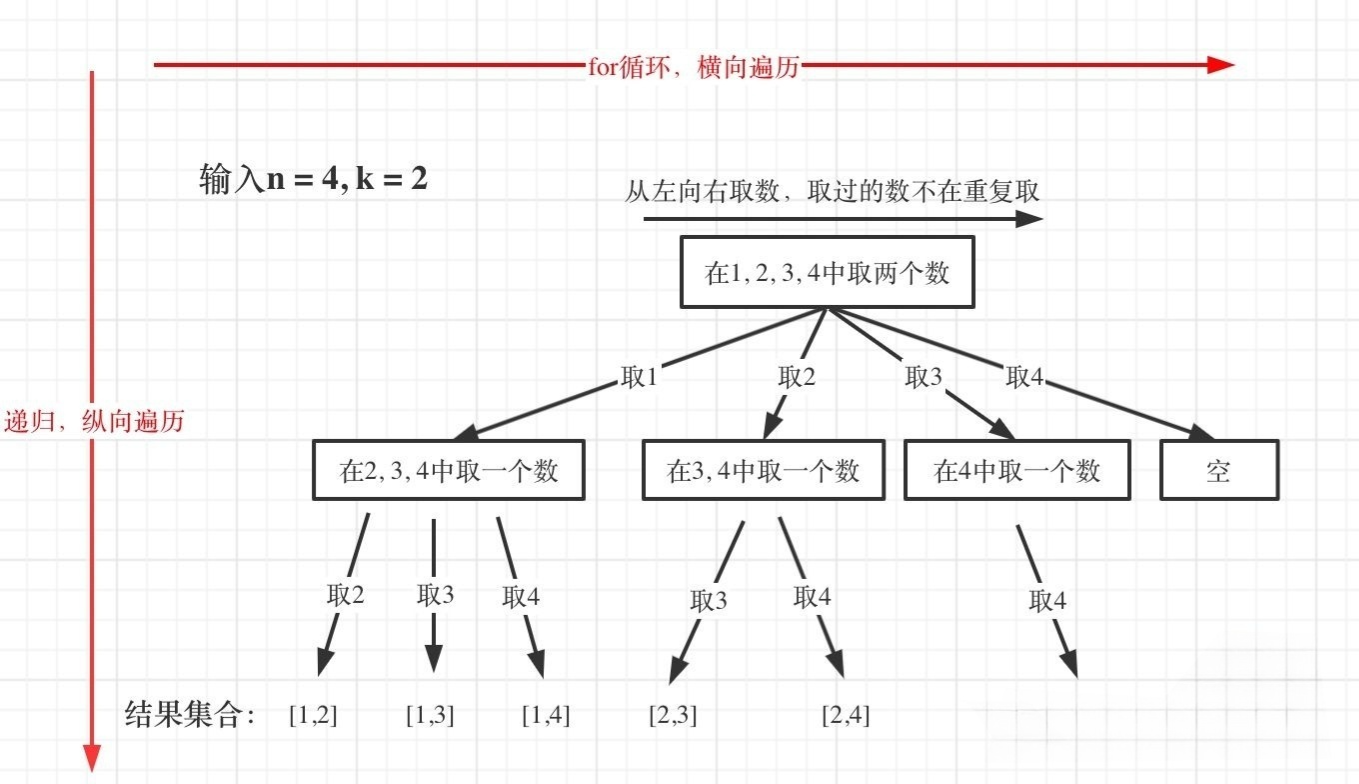
\includegraphics[width=10cm]{Figure/Figure_1.png}
            \caption{把回溯问题抽象为树形结构}
        \end{figure}
        \noindent
        针对``递归''当中的``\underline{纵向遍历}'':\par
            我这里截取了``HELLO Algo''里面``求和函数的递归过程''当中的一张图来进行粗略地说明:

        \begin{figure}[H]
            \centering
            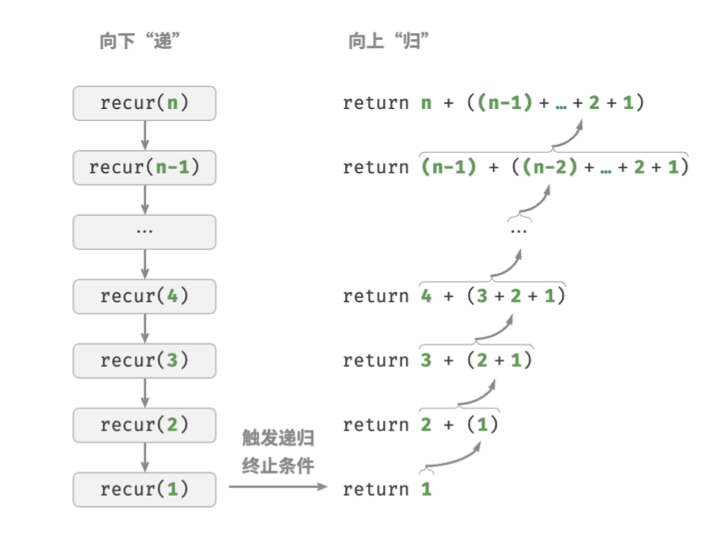
\includegraphics[width=10cm]{Figure/Figure_2.jpg}
            \caption{求和函数的递归过程}
        \end{figure}

        \noindent
        观察两张图示,我们可以非常清晰地认识到:\par
        ``回溯法''的本质就是一种``暴力搜索''
        (形式上与``for loop''类似,
        只不过一个是横向遍历,
        一个是纵向遍历而已,
        区别仅限于此)
        但我们之前在分析``回溯法''这一类``完备性算法''的时候,
        我们已经指出了``完备性算法''的一个非常大的问题 ——``\textbf{慢}''\par
            实际上,我在利用``回溯法''求解``3-SAT问题''的过程中,也确实遇到了这么个问题:\par
                (1)求解数据量比较少的测例基本没有问题\par
                (2)求解数据量比较大的测例基本上都是超时\\
            在``基于回溯法的实现''处,会展开论述这个问题\par
                很自然地,我去寻找另一类求解``3-SAT问题''的方法\ ——\ 基于``回溯法''的``DPLL算法'' \ —— \ 改进后的一种``完备性算法''
        \subsubsection{DPLL算法}
        那现在我们来重点介绍一下``\underline{\textbf{DPLL算法}}''!\par
        那么,到底什么是``DPLL算法''呢?查阅资料后,我们可以知道,所谓``DPLL算法'',
        是解决``SAT问题''的一种``完备性算法'',是对``回溯法''的一种改进。\\
        \newline
        \noindent
        这个算法主要由如下几个\textbf{核心阶段}组成:\par
            (1)当前子句可满足判断\ ——\ Current Clause Satisfied\par
            (2)布尔表达式可满足判断\ ——\ All Clauses Satisfied\par
            (3)空子句判断\ ——\ Has Empty Clause\par
            (4)单位子句传播\ ——\ Unit Propagation\par
            (5)孤立文字消去\ ——\ Pure Literal Elimination\par
            (6)使用DPLL算法(实际上就是``回溯法'')进行求解\\
        \par
        在这里做一个比较粗略的解释:
        ``DPLL算法''从本质还是``回溯法'',
        只不过我们对``回溯法''中处理``literal''的方式进行了各种优化,
        让这个``回溯法''变得更加切实可行
        \par
        关于``DPLL算法'',
        我们下面给出一张比较简略的流程图来对DPLL算法有一个比较粗略的了解:

        \begin{figure}[H]
            \centering
            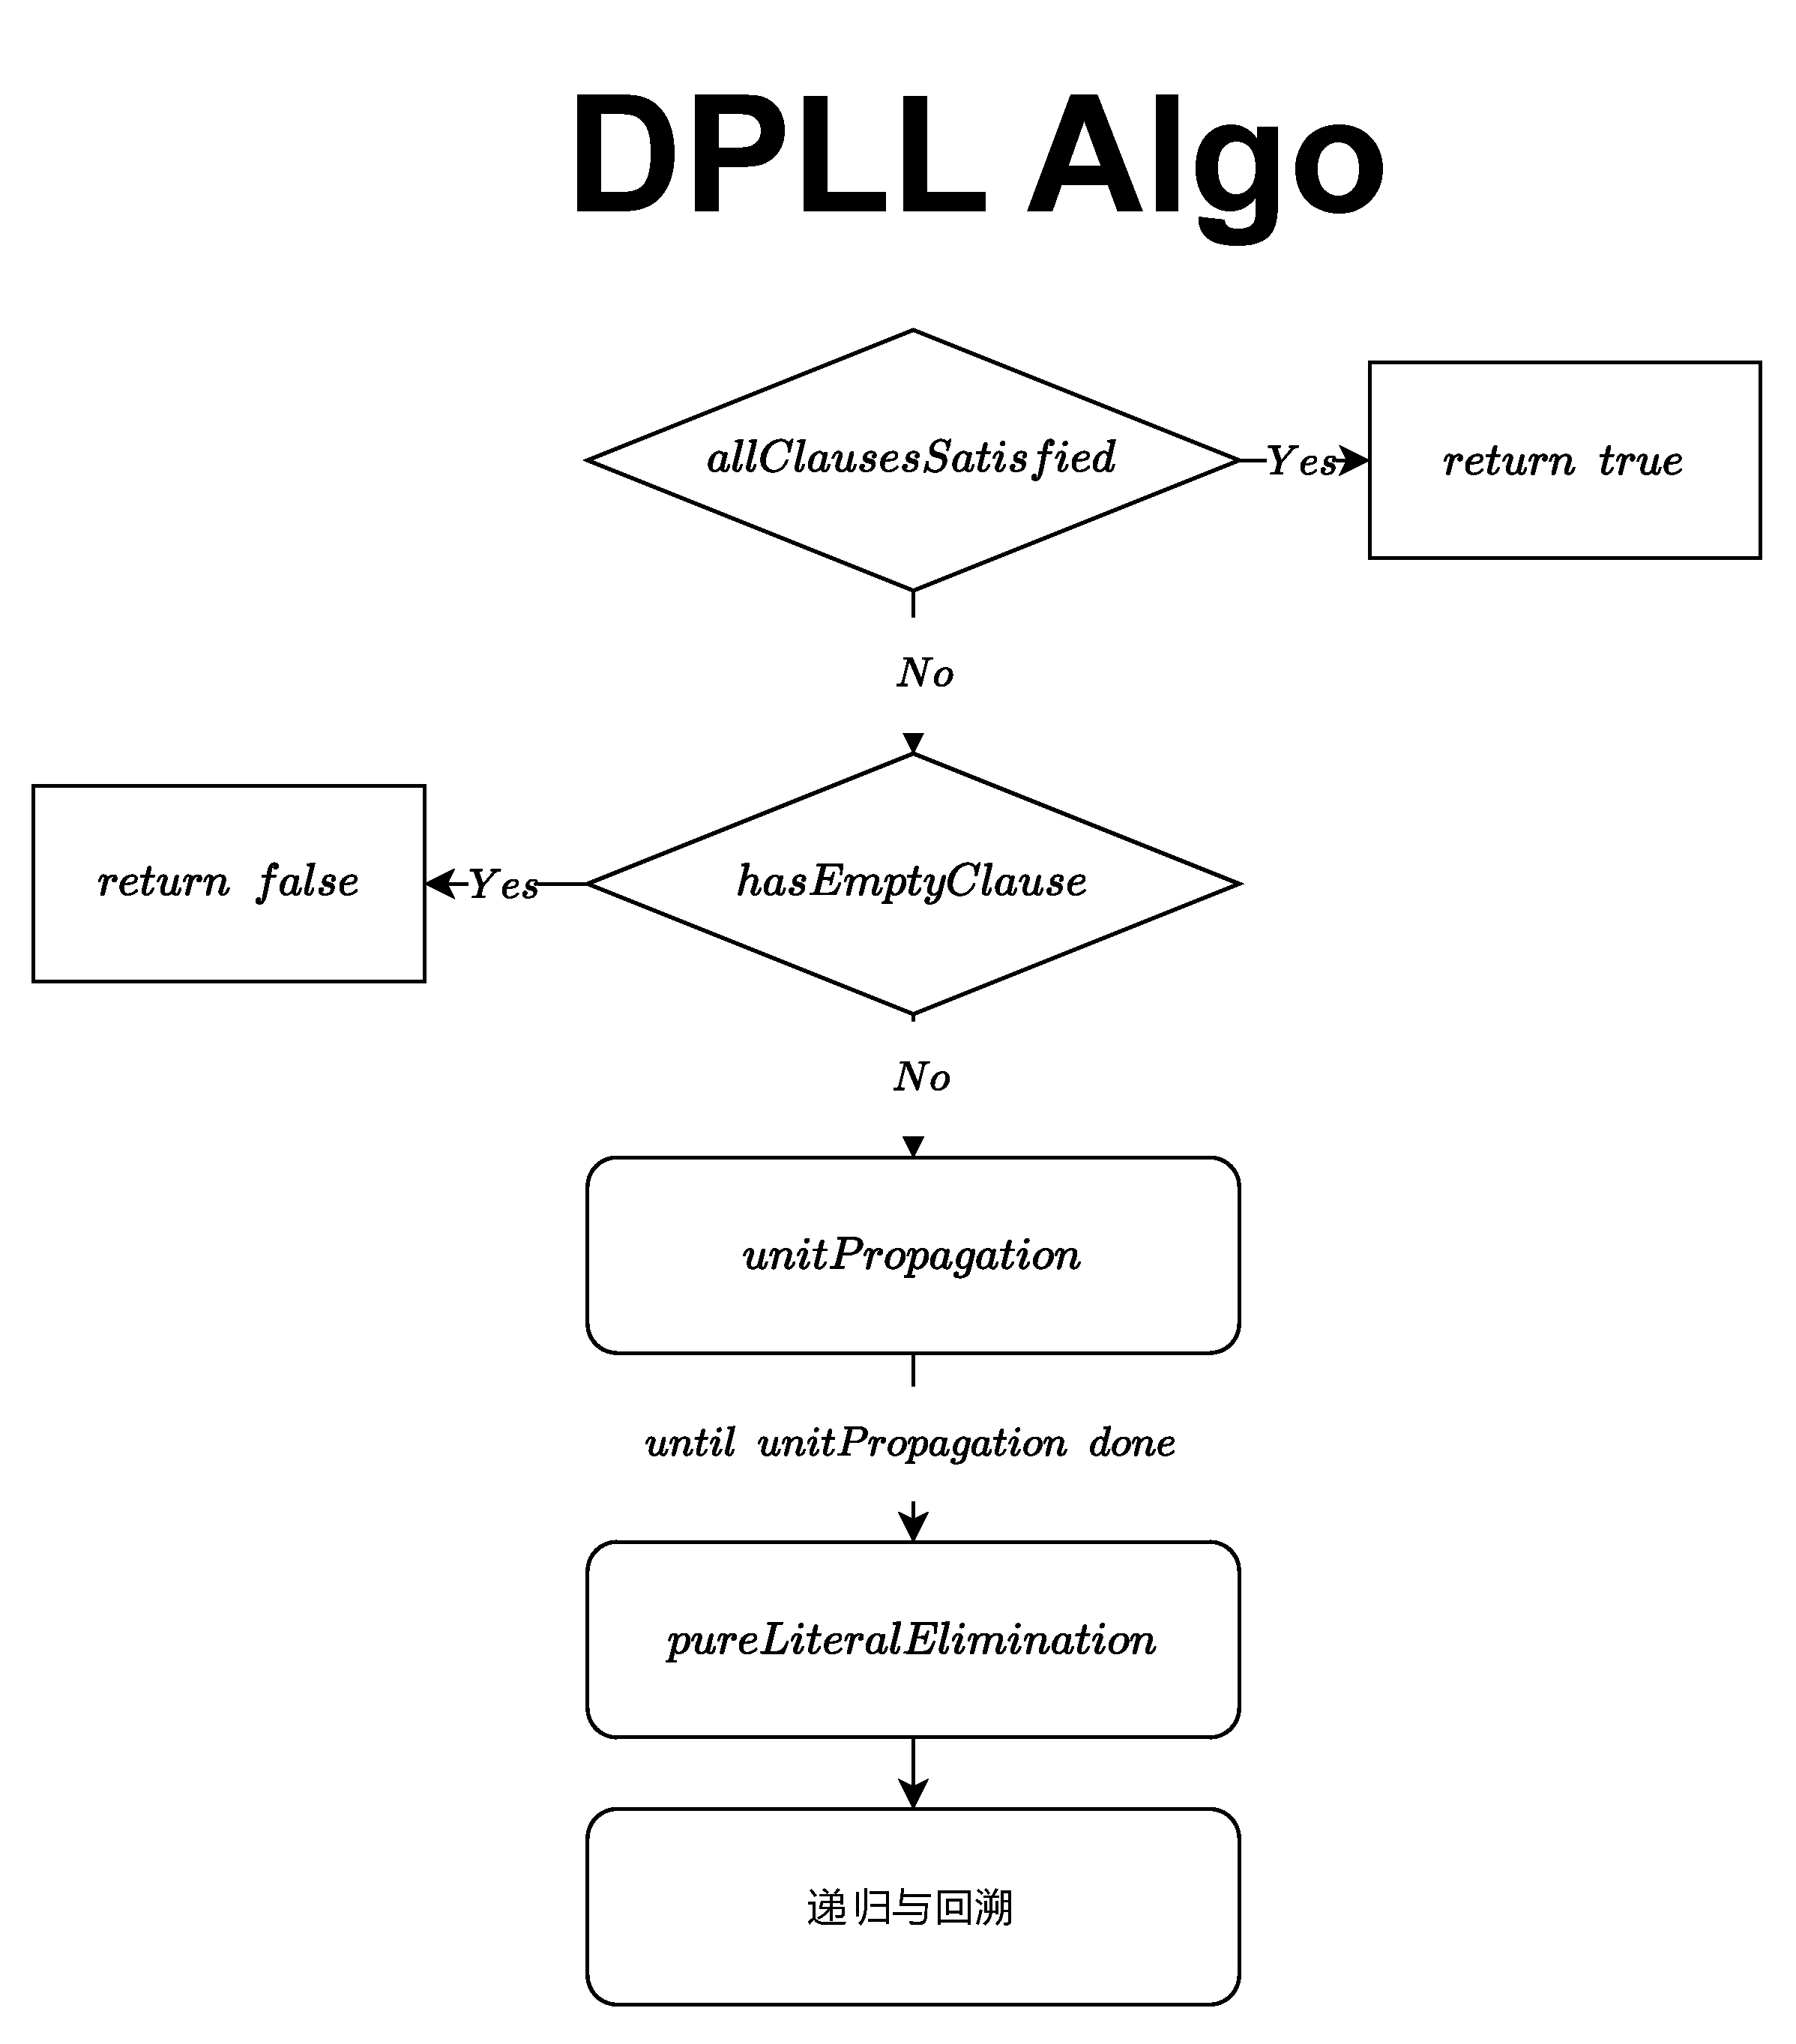
\includegraphics[width=10cm]{Figure/Figure_3.pdf}
            \caption{DPLL Algo}
        \end{figure}
        \noindent
        其实从这个流程图我们也可以看到:
        \par
        ``递归与回溯''这一步骤是在整个``DPLL算法''当中的最底部的,
        而``递归与回溯''是``回溯法''解决``SAT问题''的核心步骤,
        换言之,
        从本质上来讲,
        ``DPLL算法''就是``回溯法''
        \par
        而且从整个流程图当中,
        我们可以非常清晰地看到,
        我们在``递归与回溯''的上方加了几个预处理步骤
        \par
        至于``DPLL算法''中如何对处理``literal''方式的进行优化,
        我们会在``基于DPLL法的实现''中详细展开
        \subsubsection{WalkSAT算法}
            那么什么是``WalkSAT算法''呢?\par
            ``WalkSAT算法''是一种``非完备性算法'',
            本质上是对``贪心算法''的一种改进\par
            而我们主要基于``完备性算法''解决这个``3-SAT问题'',
            因此这里不展开讲``WalkSAT算法'',
            只是做一个简单的了解即可